To answer our research questions, we develop a tool that implements the perfect test method to find the BIC corresponding to a BFC, using regression tests as perfect tests. 
A regression test of a bug checks if this bug reappears in changes following the bug fix. 
Our hypothesis is that a regression test can be used as an approximation to the perfect test, which we will prove through our tool.
%\as{We might like to stress that we would like to understand to what extent is this operationalisation valid, i.e., to assess the gap between the construct of the "perfect test" and its operationalisation as a regression test.}
%\michel{I have extended this idea in the form of a hypothesis.}
Given a BFC and the regression test for its bug,
%\as{Implicit assumption: the regression test is part of the bug fixing commit.}\michel{We clarify that we refer to the bug and not that we assume that the BFC contains the regression test}\as{Where is this clarification?} 
the tool transplants the test to past changes, and tries to execute them, determining if they succeeded or failed. 
In order to learn how far the tests can be automatically transplanted to past snapshots of the code (RQ\textsubscript{3.1A}) and what aspects prevent transplanting the regression test into the past(RQ\textsubscript{3.1B}), we run this tool on a dataset consisting of several BFCs and their corresponding regression tests. 
To learn in which cases the BIC could be found correctly (RQ\textsubscript{3.2}), the tool identifies the BIC using the transplanted regression tests as the perfect test. 

\subsection{The perfect test method}
\label{subsec:model}

As stated by \gema~\cite{rodriguez2020bugs}, the perfect test method to find the BIC corresponding to a BFC assumes that data about changes to the source code (including the BFC and all candidates to be a BIC) can be obtained from a source code management system such as git, in which changes corresponding to fixing bugs can be identified, and related to the description of the corresponding bugs. 
The perfect test method consists of the following steps~\cite{rodriguez2020bugs}:
%\as{Are these steps coming from Gema's paper? If yes, please add a bibliographic reference.}
%\michel{The paragraph already begins with "As stated by Rodriguez-Perez et al. [31]. }

\begin{enumerate}
    \item Identify a Bug-Fixing Change (BFC) and the description of the corresponding bug.
    \item Using the change and the description of the bug, describe the bug in terms of a perfect test that would, with certainty, fail if the bug is present, or succeed if it is not (the perfect test).
    %\as{What does it mean ``describe the bug in terms of a perfect test''?}
    %\michel{These steps are a summary of Gema's work done by Jesus. Jesus, could you take a look at it?}
    \item Identify, from the past history of the code, the first change %\as{Do you mean the earliest in terms of time?``The first'' might be ill defined in presence of multiple history lines.}\michel{These steps are a summary of Gema's work done by Jesus. Jesus, could you take a look at it?} 
    for which the perfect test fails (First Failing Change, FFC).
\end{enumerate}

\gema~\cite{rodriguez2020bugs} distinguish between intrinsic and extrinsic bugs. 
%\as{Is ths Gema's distinction or has it been known in the literature before Gema?}
%\michel{Gregorio, here maybe you can shed some light for us}
\emph{Intrinsic bugs} are bugs that have been introduced by a change in the code.
In the case of intrinsic bugs, there should be a BIC, and that will correspond to the FFC: before the BIC, the bug was not present, and after it, it was present until fixed. 
\emph{Extrinsic bugs} are not introduced by a change to the source code but by an external factor, e.g., a change in an external API.
In the case of extrinsic bugs, \gema indicates that there is a first-failing moment (FFM), not present in the version control system and the FFC is the first change to the version control system after the FFM.

In the current work we focus on intrinsic bugs, and therefore for us finding the FFC will mean we found the BIC.
We will not address the detection of FFC in extrinsic bugs since regression tests cannot help us find that change and the bug dataset chosen to test our proposal (to be described in the next section) only contains intrinsic bugs.
%\as{The decision to focus on the intrinsic bugs should have been better motivated.}
%\michel{I have included the reasons why we do not address intrinsic bugs. Perhaps Gregorio can refine this decision a bit more. A very recent paper (2022): "ApacheJIT: A Large Dataset for Just-In-Time Defect Prediction" also points out Gema's study and says that it leaves out extrinsic bugs because of the difficulty of detecting them.}
For describing the bug in terms of a perfect test (2), we use regression tests. Regression tests are designed to detect if bugs are introduced in future changes, and we postulate that they are also useful to detect them in past changes.
%Regression tests are usually included in the change that fixes the bug. \as{``usually included'' refers to the assumption made before.}
Therefore, for (3) we run those tests in snapshots of the source code after changes that are previous to the BFC  in the history of changes to the source code. 
%We call running the tests on past snapshots ``transplanting the test'' to that past snapshot. 
Figure~\ref{fig:process} illustrates the transplantation process, by showing a simplified version of it: we will later discuss on this section how the BIC should be searched considering that the git history is a graph rather than a line.

\begin{figure}[h!]
  \centering    
  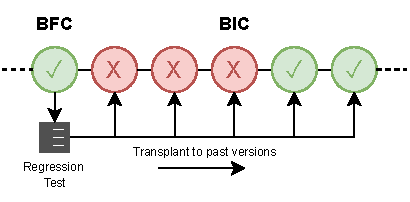
\includegraphics[width=0.8\textwidth]{pages/03-BugHunter/images/Model.pdf}
  \vspace{-0.5cm}
  \caption{Simplified process leading to finding the first failing change (FFC), by running tests in past snapshots of the project.
  \patxi{Normalmente el histórico de git se representa al revés: los commits más nuevos a la derecha y el pasado está hacia la izquierda... pero para la tesis da un poco igual}
  \michel{Asi estaba ... y Alexander me hizo darle la vuelta. Le vuelvo a dar la vueta a la figura (sobre todo para que concuerde con el gráfico similar del Chapter 3) -> TODO}
  }
  \label{fig:process}
  \vspace{-0.5cm}
\end{figure}

The paper presenting the perfect test method~\cite{rodriguez2020bugs} states that one of the main limitations of the perfect test is that being able to construct a perfect test requires a deep knowledge of the bug, how it was fixed, and the project in which it was found. 
In our case, we assume that developers writing regression tests have all this knowledge, and therefore their tests will be close to the theoretical perfect test for the bugs they fix.


\subsection{The bugs dataset}
\label{subsec:dataset}

Defects4J~\cite{just2014defects4j} is a well-known dataset with 835 bugs from 17 Java open source software projects, including only bugs located in the source code, excluding those related to the build system, configuration files, documentation or tests. It has been used as ground truth in the evaluation of several implementations of SZZ-derived algorithms~\cite{neto2019revisiting,pokropinski2022szz,wen2019exploring,an2021reducing}. 
Previous studies have identified several issues that might threaten application of SZZ-derived algorithms: e.g., links to the repositories might have  changed~\cite{lawrence2001persistence}, repositories might have been deleted, moved, made private, or their history might have been altered~\cite{bird2009:promises_perils_git}.
However, Defects4J includes the whole source code management repositories of each project, avoiding the problems mentioned above.
All but one of the repositories in Defects4J are git repositories, which is the source code management we will target in our study.

% Defects4J is not only a dataset, but a whole framework for working with the repositories and bugs it includes. \as{This seems to contradict the first sentence of this section ``Defect4J is a well-known dataset...'' Please rephrase.}
% It provides a command-line tool for extracting information related to a bug (e.g., the fixing commit, the bug report, and the regression test), \as{This is odd: so far there has been no discussion that Defect4J contains fixing commits, this point will be made only in the next paragraph. Maybe move this paragraph further downwards?} get a copy of the corresponding repository, and other useful tasks, which makes it easy to work with the dataset. \as{The last fragment ``and other useful tasks...'' does not seem to be useful.}

Every bug included in Defects4J identifies the change (commit) fixing it (its BFC), and refers to a publicly available bug report which details the nature of the bug.
From here on we refer to changes as commits, since we will focus on git repositories.
% \as{It seems that we are using the words ``change'' and ``commit'' interchangeably. Moreover, we are also calling the same thing a ``node''. Can we maybe select one of the terms and use it consistently?}
% \michel{Now, from the second paragraph of Section~\ref{subsec:dataset} where the term commit is stated as the "change" defined above, only the term "commits" is used. The term "change" is kept in the Section~\ref{subsec:model} to be consistent with Gema's work.}
% \as{OK, we might like to add a sentence like ``From here on we refer to changes as commits'' or something similar.}
This bug report will be required when manually evaluating the detected BICs.
Therefore, the dataset complies with step (1) of the perfect test method. 
Associated with each bug there is also a regression test, included in the BFC, that exposes the bug. 
The dataset also provides its own commands to compile the code and execute the test in this commit. 
We will use this regression test as a perfect test for the bug, therefore complying with step (2) of the perfect test method.
Although the regression tests included in Defects4J have been reviewed by the authors of the dataset and emphasize in their tool that they have left out any flaky test, we have run each test 3 times in the BFC to verify that their results do not differ, and therefore we avoid including non-deterministic tests in the experiment.

The dataset does not include information about the commit that introduced the bug (if any), which we would need to verify that the result of step (3) of the perfect test method found the right change. 
However, the dataset provides a specific (synthetic) snapshot of the code without the fix (that is, with the bug present), in which we can check that the test fails. 
This supports our assumption that the regression tests identified in the Defects4J dataset can be used as perfect tests.

% \as{It seems that the previous paragraphs where describing the dataset as is, while the remaining part of the subsection discusses what we have done to it (excluding some parts). Would it be a good idea to split 3.2 into 3.2.1 and 3.2.2?}
% After examining the dataset, we found that the projects in it use different build systems, \as{At this point it is not clear why is it even important to know what build systems are used by the projects. Consider making this explicit.} among which we identified Maven, Gradle and Ant (all common Java build systems).\as{Is the comment ``all common Java build systems'' really necessary?}
%  In our case, we decided to build snapshots, and execute the transplanted tests, only with Maven or Ant. 
% Maven is one of the most widely used build systems in Java and offers the least problems when reproducing a build~\cite{sulir2016quantitative}. 
% Additionally, we also use Ant because many projects using Maven had used Ant at some moment in the past (Maven replaced Ant as the build system in many projects, including some in the dataset\as{Do we have a reference to support the claim that many projects moved from Ant to Maven?}). 
% Therefore, for transplanting tests to any commit in the past history of projects using Maven, in some of them we also need to support Ant. 
% Including Gradle didn't significantly increase our chances\as{I am not sure that the phrasing in terms of chances is precise; maybe rephrase?} of building snapshots and running tests, as only one of the projects selected uses Gradle, and this project also offers support for Ant, so it is included in our study.

From the whole Defects4J collection of projects, we excluded project Chart because it uses Subversion~\footnote{\url{https://subversion.apache.org/}} as version control system. 
We focus only on projects that use Git. 
As a result, we included in our experiment 16 projects out of the 17 found in Defects4J, with a total of 809 bugs of the initial 835 bugs.
Table~\ref{table:dataset-table} shows a brief description of the selected projects: the number of bugs it contains reported by the dataset, the number of stored commits, the dates for the first commit of the project and the last one (the last commit does not correspond to the last one in the official repository, since the projects in the dataset are stored as a copy of the git repository at a specific point in time). 
It should be noted that this dataset was extended in 2020, based on the original 2014 dataset~\cite{just2014defects4j}.

\begin{table}[]
    \caption{\label{table:dataset-table} Description of the projects used from Defects4J}
    \resizebox{\textwidth}{!}{%
        \begin{tabular}{|r|r|r|r|r|}
            \hline
            \textbf{Project} & \textbf{\# of bugs} & \textbf{\# of commits} & \textbf{First Commit} & \textbf{Last Commit} \\ \hline
            Cli              & 39                  & 914                    & 2002-06-10            & 2019-03-25           \\ \hline
            Closure          & 174                 & 2,898                   & 2009-11-03            & 2013-12-13           \\ \hline
            Codec            & 18                  & 1,795                   & 2003-04-25            & 2019-04-23           \\ \hline
            Collections      & 4                   & 3,091                   & 2001-04-14            & 2019-03-25           \\ \hline
            Compress         & 47                  & 2,682                   & 2003-11-23            & 2019-03-25           \\ \hline
            Csv              & 16                  & 1,290                   & 2005-12-17            & 2019-04-14           \\ \hline
            Gson             & 18                  & 1,476                   & 2008-09-01            & 2019-11-05           \\ \hline
            JacksonCore      & 26                  & 1,724                   & 2011-12-22            & 2019-04-24           \\ \hline
            JacksonDatabind  & 112                 & 5,241                   & 2011-12-22            & 2019-05-15           \\ \hline
            JacksonXml       & 6                   & 949                    & 2010-12-30            & 2019-05-05           \\ \hline
            Jsoup            & 93                  & 1,261                   & 2010-01-17            & 2019-07-04           \\ \hline
            JxPath           & 22                  & 598                    & 2001-08-23            & 2018-05-15           \\ \hline
            Lang             & 64                  & 3,596                   & 2002-07-19            & 2013-10-10           \\ \hline
            Math             & 106                 & 4,913                   & 2003-05-12            & 2013-10-16           \\ \hline
            Mockito          & 38                  & 3,262                   & 2007-11-15            & 2016-08-02           \\ \hline
            Time             & 26                  & 1,718                   & 2003-12-16            & 2013-12-04           \\ \hline
        \end{tabular}
    }
\end{table}

%Defects4J can be used to check if the operationalization of the perfect test method by using regression tests actually detects the commit that introduced each of the bugs. \as{It seems that the previous sentence is much more precise than the current phrasing of the RQ. Maybe rephrase the RQ?}
% For this, we check if step (3) of the method, which finds the FFC for the test, actually detects the BIC for the given bug.

\subsection{Transplanting the test to the past}
\label{subsec:transplant} 

Following the process shown in Figure~\ref{fig:process}, we have designed and implemented a Python tool that automates all the necessary tasks to transplant the regression test to the commits corresponding to past changes, and run it to determine if it fails or succeeds. 
For each bug in our subset of the dataset, it takes the following steps:

\begin{enumerate}
  \item \textbf{Extract information.} 
    By using the command-line tool provided by Defects4J, extract the fix commit, bug report and regression test for the bug.
  \item \textbf{Set up the repository.} 
    By using the Defects4J command-line tool, obtain a copy of the git repository of the project corresponding to the bug.
  \item \textbf{Execute the regression test on the fix commit.} 
    This will ensure that the test actually succeeds for this snapshot, which means that it succeeds when the bug is fixed (if not, the test would not check properly, as the perfect test method states). For this, the tool checkouts the snapshot corresponding to the bug fixing commit (BFC), and runs the regression test on it.
    In this step, the file containing the test is stored, in order to be transplanted into the previous snapshot (the test method, as well as the file name and the path where it is located is provided by the dataset).
  % \item \textbf{Execute the regression test in the commit prior to the fix.}
  %   This will ensure that the test actually fails in this snapshot, confirming that it detects the bug properly (if it succeeds, the test is not detecting the bug properly, in the sense defined by the perfect test method). 
  %   For this, checkout the snapshot corresponding to the previous commit, transplant the regression test, and try to run it.
  %   We refer to transplanting as placing the file containing the test (copied from the BFC) in the original path (recreating the original directory if necessary).
  \item \textbf{Execute regression test on all previous commits.}
    This will allow us to find the first failing change (FFC), which as we discussed, in the case of intrinsic bugs, will be the BIC that we are looking for. For this, the tool checkouts each of those past commits, transplants the test to each of them, and runs it in each of them. 
    The FFC will be the first one that fails after the last one that succeeds. 
    %The list of past commits is obtained through the command \textit{git log --reverse}, run from the BFC.
\end{enumerate}

In the steps that execute regression tests, the tool follows this procedure:
\begin{inparaenum}[\bf(1)]
\item \textit{checkout the corresponding commit},
\item \textit{transplant (copy) the regression test},
\item \textit{compile the source code},
\item \textit{compile the regression test}, and
\item \textit{execute the regression test}.
\end{inparaenum}
For compiling and executing we decided to use standard Maven and Ant commands, since the command provided by Defects4J only works with some specific commits (in the BFC and in a synthetic commit where the bug is present), and we needed to build and run the test on any of them (see previous discussion on finding the FFC at Section~\ref{subsec:model}). 
%However, we used the copy of external libraries provided with Defects4J, thus avoiding problems due to some of them no longer being available.

When the tool finishes all actions for a given bug, it reports the results of executing the regression test (if that was possible) for all commits prior to the BFC. These results include the success or failure of the different phases: building the source code, building the transplanted test code, running the regression test, and the result (fail or success) of running the test. 
In order to know the reasons for failures, the tool also keeps a log of the execution of each step.

In order to measure how far a test can be transplanted to the past and answering \textbf{RQ\textsubscript{3.1A}}, it is necessary to define a metric that allows us to measure how far we can transplant a regression test. 
We propose the \textit{Transplantability} metric. 
For a given bug for which we have a test that detects it, we consider all commits that are ancestors of the BFC, in chronological order, and from this ordering we will find a commit $n$ which is the oldest at which the test can be transplanted and executed. 
We define \textbf{Transplantability (in days)}, $T_{days}$ as the number of days between commit $n$ and the BFC. 
In the same way, we define \textbf{Transplantability (in commits)}, $T_{commmits}$ as the number of commits between 
%\as{What does ``between'' mean for a tree? Is there always a branch between $n$ and the BFC?}\michel{We consider the chronological order (as stated above), not the branches.} \as{Where did we say this? Do we want to somehow integrate this chronological idea in the definition of $T_{commmits}$? Is it not odd to somehow count commits belonging to completely different branches?}
%\michel{We rephrased the first part of the paragraph to explain that the commits are traversed in chronological order.}
commit $n$ and the BFC.
The two different ways of quantifying, together, are intended to give a more comprehensive view of how far we can transplant a test into past commits.

In Chapter~\ref{chapter:buildability} we had already stated that at least in the compilation of the source code we may face problems that will prevent us from continuing with the experiment. 
We also consider the likelihood that errors may also occur in the compilation of the regression test and in the execution of the test itself (i.e., that the test does not generate a report indicating whether the test passes or fails).

Problems related to compilability of source code, the compilability of the regression test code (the transplanted test), and the runnability of the regression test will be studied in order to answer \textbf{RQ\textsubscript{3.1B}}. 
To further understand these problems, we introduce three definitions: source code compilability, transplanted test compilability, and transplanted test runnability.

\textbf{Source code compilability} is defined as the percentage of snapshots in the past history of the BFC that could be successfully compiled.
This metric was originally defined by Tufano et al.~\cite{tufano2017there} and used in Chapters~\ref{chapter:buildability} and~\ref{chapter:testability}.
These previous studies took as reference commit the last one in the repository (the most recent one), considering as the commit history of the project all the commits previous to this one. 
In this chapter we will use as reference the BFC commit to define the commit history for each bug. In this way, we will calculate the Source code compilability of the commits previous to the BFC.

\textbf{Transplanted test compilability} is similar, but for the transplanted test: the percentage of snapshots in the past history of the BFC in which we could compile the transplanted test. 
These parameters let us know how often the reason for not being able of running the transplanted test was not being able to compile the test itself or compiling the source code in each of the snapshots.

\textbf{Transplanted test runnability} is defined as the percentage of snapshots in the past history of the BFC in which we could run (execute) the transplanted test without errors, producing a ``success'' or ``fail'' result, as stated in Chapter~\ref{chapter:testability}. The larger the test runnability, the more commits in which we could run the test. If it is 100\%, the perfect test method can be run for the whole history before the BFC. When test runnability is not 100\%, for some commits we cannot assess if the test fails or succeeds (because it doesn't run). Depending on success and fail in other commits, maybe we have to add the commit to the list of candidate BICs without being able of be more conclusive about it. Therefore, the transplanted test runnability shows how successful is the transplantation of regression tests to past commits.

\subsection{Identifying the Bug Introducing Change}
\label{subsec:identify-bic}

From the results obtained after transplanting the regression test on the commits prior to the BFC we can seek to locate the BIC.
At this point, we can revisit what ``all previous commits'' from Step 4 mean. 
In Figure~\ref{fig:process} we present the history of commits as linear. 
However, in a real git repository the commit history might not be linear: there are development models (as GitFlow~\footnote{\url{https://nvie.com/posts/a-successful-git-branching-model/}}) with git in which development is done in parallel branches, which are merged when convenient. 
Therefore, the history of a project can be considered as a directed graph. 
The previous theoretical model contemplated only a linear history of commits, which limits the understanding of this history. The consideration of the history as a graph to further refine the BIC search is a contribution of this work.
Each node represents a commit that will point to the commits that precede it (its parents), which can be one or more.

With this in mind, we developed Algorithm~\ref{alg:bic} to detect the BIC in this graph. 
This algorithm receives as parameters the graph, annotated with the result of running the tests (its status, which can be success, fail or error) and the identification of the BFC in that graph. 
%This algorithm returns the list of candidates to be the BIC. 
This algorithm traverses the graph using a depth-first search~\cite{cormen2022depthfirstsearch}, starting with an empty list of candidates, and trying to find the list of candidates to be the BIC, according to the perfect test method. 
For that, the algorithm finds the node $n$ in which the test fails and which preceding nodes succeed (success parents), which would make $n$ a candidate to be the BIC.

Since for some nodes we could not run the test (because it could not be compiled, it did not run, or the source code could not be compiled), we must consider that in these nodes the tests may or may not be executed successfully.
%Therefore, the algorithm finds all nodes in which the test fails, or cannot be run, and in all nodes preceding these nodes the test succeeds, or cannot be run. 
%All the nodes found by the algorithm would be the candidates to be the BIC.
\begin{footnotesize}
    \begin{algorithm}[t!]
        \caption{Algorithm to detect bug-inducing commits}\label{alg:bic}
        \SetKwInOut{Input}{Input}
        \SetKwInOut{Output}{Output}
        \SetKwInOut{Precondition}{Precondition~}
        \Input{A $\mbox{\sl graph}$ (commit history) and the $\mbox{\sl bfc}$}
        \Output{A list of candidates for BIC}
        \Precondition {The $bfc$ status (the output of the regression test) must be success
        % \as{I understand the intention but ``status'' does not seem to be defined. }
        % \michel{I clarify what ``status'' is at text}
        % \as{It might be a good idea to explain ``status'' here such that the algorithm becomes self-contained?}
        }

        $candidates \gets []$\;
        $queue \gets [bfc]$\;
        $visited \gets [bfc]$\;
        $temp\_candidates \gets []$\;
        
        \While{$ NotEmpty(queue) $}{
            $n \gets GetFirst(queue)$\;
            \If{hasFailStatus(n)}{
                $candidates \gets []$\;
            }
            $parents \gets GetParents(graph, n)$\;
            $successParents \gets True$\ \Comment*[r]{Control if all parents are success} 
            % \as{What does $successParents$ mean?}
            % \michel{I clarify at text}
            \If{$ isEmpty(parents) $\Comment*[r]{Reach first commit}}{
                    \eIf{size(queue) == 0}{
                        $break$\;
                    }{
                        $continue$\;
                    }
            }

            \For{$p \in parents$}{
                $successParents \gets successParents \And hasSuccessStatus(p)$\;
                \If{$ \neg hasSuccessStatus(p) $}{
                    \If{$ hasErrorStatus(p) $}{
                        $AddItem(candidates, n)$\;
                    }
                    \If{$ p \notin visited $}{
                        $AddItem(queue, p)$\;
                        $AddItem(visited, p)$\;
                    }
                }
            }
            \If{$ successParents \And \neg hasSuccessStatus(n) $}{
                \eIf(){$ hasFailStatus(n) $}{
                    \Return{$[n]$}\; 
                }{
                    $AddItem(candidates, n)$\;
                    
                    \eIf(){IsEmpty(queue)}{
                        \Return{$candidates$}\;
                    }{
                        $temp\_candidates \gets candidates$\;
                    }
                    
                }
            }
        }
        \Return{$temp\_candidates$} 
    \end{algorithm}
\end{footnotesize}

The algorithm operates under the following assumptions: (1) all the ancestors of the BIC are success commits, until the beginning of the history of the project, or until the features on which the test is built are introduced; (2) in the case of a commit with two or more parents, which generate branches, the BIC can only be in one of these branches.
The first assumption is based on the definition of the BIC: the first commit where the bug manifests, which following the perfect test method, means the first commit where the test fails. In other words, in snapshots previous to the BIC the bug is not present, and therefore the test, if it can be run, should succeed. The test may not run if it is designed on top of some feature (e.g., some function) that does not exist for some snapshot, because it was not yet implemented.
The second assumption is based on the unlikeness that the same bug (which is fixed by a single fix commit) is introduced in two different branches. 
% For any given bug, it may happen that the test does not succeed in the BFC. 
% This may happen because the source code or the test is not compilable, in which case we can say nothing: we just do not have enough evidence to guarantee that the test actually succeeds for the BFC, and therefore we do not run it (we considered this as a precondition for identifying the BIC). We will consider that we do not have enough data for this bug, and will ignore it in our study.

Our algorithm has as a precondition that the regression test can be run and gives a successful result in the BFC.
If this precondition is fulfilled, we can run the algorithm, and come with two different outcomes:

\begin{itemize}
\item \textbf{The test succeeds in some preceding commit.}
  We should find at least one parent commit of the BFC for which the test fails (we should have at least one snapshot where the bug is present). 
  Following the ancestors of those commit that fail, we eventually find one that succeeds. 
  If we find a commit $n$ where the test does not succeed, but it succeeds for all its parents, then $n$ should be considered the commit that introduced the bug. 
  In this case, the algorithm found a single candidate and returns it. If we find a commit $n$ where the test cannot be compiled, and it succeeds in all its parents, then all commits between $n$ and $m$, being $m$ the first descendant of $n$ where the test can be compiled and fails, are considered candidates. 
  In this case, we have found several candidates, and we cannot decide which one is exactly the BIC because we cannot run the test in them, but we know the BIC should be one of them.
\item \textbf{The test does not succeed in any precedent commit.}
  In this case, we should assume that the bug was always in the code, since the functionality tested by the test was introduced or that we cannot run the test for some reason (i.e., we are not able to compile the source code). In any case, we cannot find the BIC: either it doesn't exist, or it is hidden because we cannot run the test, so the algorithm returns an empty list of candidates.
\end{itemize}

As an example of how the algorithm works, Figure~\ref{fig:bug41} represents the commit history for Bug 41 of the JacksonDatabind project from Defects4J dataset. 
The figure includes only commits relevant to understanding how the algorithm finds the BIC, and consecutive commits (without forks or merges) of the same color have been reduced to one. 
Each commit is identified with a number, whose value simply indicates its chronological position with respect to the fix commit (BFC) in order to be able to refer to them.
Colors in the figure show if the regression test succeeds (green~\checkmark) or fails (red~$X$).

\begin{figure}[ht!]
  \centering   
  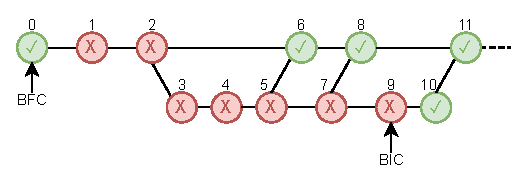
\includegraphics[width=\columnwidth]{pages/03-BugHunter/images/Databind_41.pdf}
  \caption{Visual representation of the results of the experiment for Bug 41 of JacksonDatabind project.\michel{Darle la vuelta}}
  \label{fig:bug41}
\end{figure}

In this figure we can see how Commit 2, although it has a green parent (Commit 6), cannot be considered as BIC, since it has another parent (Commit 3) where the bug is present. Following the ancestors chain, the algorithm will at some point find Commit 9, which is red, but for which all parents are green (in this case, only Commit 10). 
%All ancestors of Commit 10 are green too. 
Therefore, the candidate list in this case will include only Commit 9.

% As stated before, all the is fully automated in a tool implemented as a set of Python scripts (see Figure~\ref{fig:tool}). First, information about the bug (the BFC, the regression test that reveals the bug and the link to the test report) and the corresponding Git repository are extracted by \textit{ExtractBugsD4J.py} using the command-line tool provided by Defects4J (D4J). Then, the regression test is run on the BFC and all the commits preceding it, using \textit{RegTestExecutor.py}. The results of the building process for each commit, and the result of running the test is recorded. \textit{CommitGraph.py} uses these results to produce a labeled graph (with labels showing the results of building and test running), which is fed to \textit{Analysis.py}, which runs the Algorithm~\ref{alg:bic} to find BIC candidates.

% \begin{figure}[t!]
%     \centering   
%     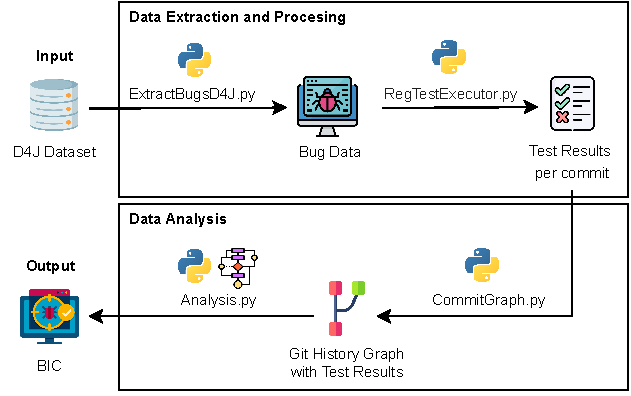
\includegraphics[width=\columnwidth]{images/RegressionTool.pdf}
%     \caption{Processes carried out by the tool. All scripts and documentation for the tool are available in the reproduction package (See `Reproducibility' section at the end of the paper).}
%     \label{fig:tool}
%     \vspace{-0.5cm}
% \end{figure}

%\as{This section seems to be too lengthy...}
%\michel{Huge refactor has been performed}

\subsection{Manual validation}
\label{subsec:manual}

To ensure that the results of our study can be considered as ground truth, we verified them by performing a manual validation of the BICs detected for each analyzed bug. For this purpose, we performed the following steps for each BIC detected:

\begin{itemize}
    \item Check and understand the bug report
    \item Check and understand the fixed functionality in the BFC.
    \item Check and understand the changed functionality in the candidate BIC
    \item Check the output of the test run
\end{itemize}

Following these steps, we categorized the BICs found in our study as true positives or false positives, using only true positives as the ground truth in order to generate a validated dataset of BICs.

%%% Local Variables:
%%% mode: latex
%%% TeX-master: "../paper"
%%% End:
